
\chapter{Oltre JavaScript - Nuovi Linguaggi per lo sviluppo di Web App Complesse}

Dal momento che il linguaggio JavaScript \'e risultato troppo limitato per lo sviluppo delle applicazioni web che negli anni sono diventate sempre pi\'u grandi e complesse, sono stati sviluppati dei framework con l'obiettivo di aiutare lo sviluppatore nella gestione e nell'organizzazione del codice.
Un'altra valida alternativa per il programmatore \'e servirsi di nuovi linguaggi di programmazione pi\'u evoluti di JavaScript, i quali permettono al codice scritto di essere convertito in semplice JavaScript.Quest'ultimo viene quindi utilizzato come una sorta di codice assembly su cui sviluppare applicazioni con linguaggi di livello pi\'u alto.
I primi a proporre un linguaggio di questo tipo sono stati Google (Dart) e Microsoft (Typescript).



%
% Commento: questa ? la prima sezione
%
\section{Dart}

Dart, presentato per la prima volta ad ottobre del 2011, \'e un linguaggio di programmazione per il web sviluppato da Google con l'obbiettivo di sostituire javascript nello sviluppo di applicazioni basate sul web.
Il linguaggio Javascript infatti ha alcune limitazioni impossibili da risolvere evolvendolo ulteriormente ed il team di Google ha deciso di optare per la creazione di un linguaggio nuovo e pi\'u moderno, in grado di risolvere queste limitazioni e di offrire prestazioni migliori.

Le caratteristiche pi\'u importanti di Dart sono le seguenti:

\begin{enumerate}
\item \'E un linguaggio orientato agli oggetti di tipo Class-Based
\item Supporta l'ereditariet\'a, ma solo da una classe. Non supporta quindi l'ereditariet\'a multipla.
\item Permette la scrittura di codice non tipizzato.
\item Rende disponibili due modalit\'a di esecuzione, una per facilitare il debug e l'altra per migliorare le prestazioni.
\end{enumerate}

\subsection{Costruttori}
Dart \'e un linguaggio che supporta le classi, di conseguenza prevede l'utilizzo di un costruttore; in particolare ammette il named constructor e il factory constructor.
Questo linguaggio non supporta l'overloading, di conseguenza, al fine di poter definire pi\'u di un costruttore all'interno di una classe, \'e stato definito il named constructor.
Nella figura ~\ref{dart_named_costructor} si pu\'o notare come sia possibile istanziare l'oggetto CoppiaDiNumeri anche attraverso il costruttore CoppiaDiNumeri.aZero() grazie al Named constructor.
\begin{figure}[tp]
    {\begin{center}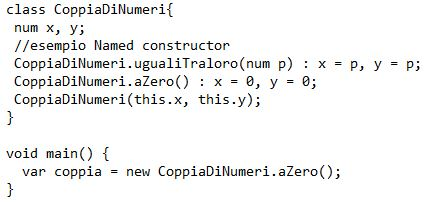
\includegraphics[width=12cm]{figure/Dart_named_costructor.jpg}\end{center}}
\caption{Il codice mostra l'utilizzo del named costructor in Dart\label{dart_named_costructor}}
\end{figure}

Dart supporta nativamente l'utilizzo del Factory Pattern tramite il costruttore di tipo factory, nella figura ~\ref{Dart_factory_costructor} \'e riportata una classe che contiene un costruttore di questo tipo.
In questa porzione di codice la variabile altraLetteraX dovrebbe istanziare un oggetto differente dalla variabile letteraX ma, dal momento che esiste gi\'a un oggetto di tipo Lettera con il nome 'X', la seconda variabile conterr\'a l'oggetto creato dalla prima.
\begin{figure}[tp]
    {\begin{center}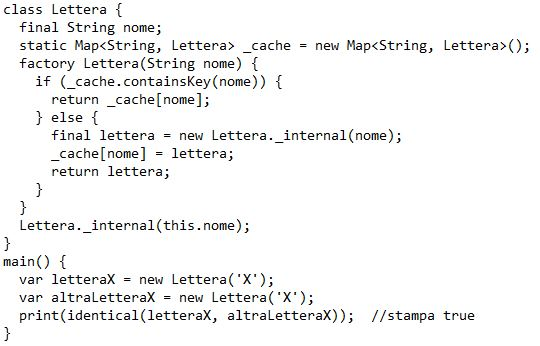
\includegraphics[width=15cm]{figure/Dart_factory_costructor.jpg}\end{center}}
\caption{Il codice mostra l'utilizzo del factory costructor in Dart\label{dart_named_costructor}}
\end{figure}

\subsection{Funzioni}

Esistono tre diverse notazioni per le funzioni nel linguaggio Dart: named functions, anonymous functions e arrow functions.
Nella figura ~\ref{funzioni_Dart} \'e possibile osservare la sintassi delle tre funzioni: il primo metodo \'e molto simile agli altri linguaggi come Java, il secondo metodo prevede una funzione nella quale non \'e specificato il nome e il tipo di ritorno ed il terzo valuta l'espressione e restituisce il risultato di essa.
Normalmente le funzioni anonime sono utilizzate per la gestione di eventi e callback e le arrow ogni volta che \'e possibile utilizzarle, nei restanti casi si utilizzano le funzioni con nome.
\begin{figure}[tp]
    {\begin{center}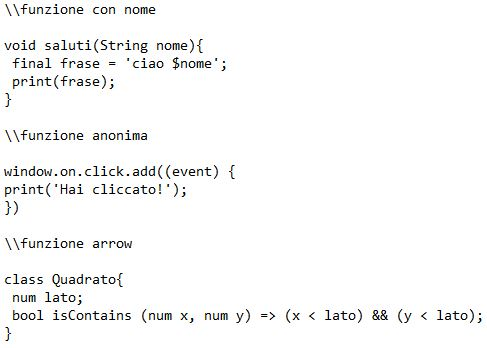
\includegraphics[width=12    cm]{figure/funzioni_Dart.jpg}\end{center}}
\caption{Il codice mostra i 3 tipi di funzioni ammessi da Dart\label{funzioni_Dart}}
\end{figure}

\subsection{Integrazione con html}
Tutti i linguaggi orientati al web hanno la necessit\'a di poter interagiore con le pagine html, nel caso di Dart \'e possibile inserire il codice dentro al tag script, settando il valore dell'attributo type a "`application/dart"'.
L'importazione di script esterni \'e permessa grazie al comando \#surce, mentre le librerie possono essere incluse con \#import.
\begin{figure}[tp]
    {\begin{center}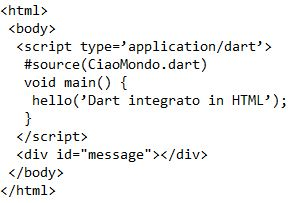
\includegraphics[width=8cm]{figure/Dart_html.jpg}\end{center}}
\caption{Il codice mostra l'integrazione di Dart in un file html\label{html_Dart}}
\end{figure}
Nella figura ~\ref{Dart_html} si pu\'o osservare un esempio di integrazione di Dart in un file html e di come sia possibile importare uno script esterno.

\subsection{Compilazione}

Nel linguaggio Dart, il codice pu\'o essere compilato in due diverse modalit\'a: controllata o di produzione. Nel primo caso, vengono eseguiti maggiori controlli ed \'e consigliato usarla in fase di sviluppo e test.
Con la modalit\'a produzione, invece, Dart compila il codice con la migliore efficienza possibile, ignorando alcuni comandi utili solo in fase di progettazione (es specificare il tipo di variabile) per ottenere un prodotto pi\'u performante; questa modalit\'a \'e consigliata per la creazione del prodotto finale.
Per poter essere eseguito sfruttando al massimo le sue performance, Dart necessita di una particolare virtual machine all'interno del browser, questo lo ha reso un linguaggio meno versatile rispetto alla concorrenza, dal momento che questa VM \'e poco diffusa.
In alternativa \'e possibile convertire il codice in puro JavaScript, al costo di una diminuizione delle prestazioni.





\section{TypeScript}
TypeScript \'e un linguaggio di scripting proposto da Microsoft nel 2012, con l'obbiettivo di risolvere le limitazioni del linguaggio JavaScript.
A differenza di Dart, si pone come superset di JavaScript, \'e quindi pienamente retrocompatibile con il linguaggio di scripting, garantendo agli sviluppatori bassi tempi d'apprendimento e fornendo la possibilit\'a di riutilizzare codice e librerie scritte in JavaScript.

Tra le caratteristiche pi\'u interessanti di questo linguaggio emergono le seguenti:

\begin{enumerate}

\item Ereditariet\'a e polimorfismo, sono possibili grazie alla natura del linguaggio che ammette le classi.
\item Compatibilit\'a con tutte le librerie JavaScript.
\item	Possibilit\'a� di utilizzare la tipizzazione statica opzionale.
\item Supporto nativo alla logica dei moduli.

\end{enumerate}

Anche se pi\'u recente rispetto a Dart, ha avuto subito un enorme successo grazie alla sua sintassi molto simile a JavaScript.

\subsection{Classi}
\begin{figure}[tp]
    {\begin{center}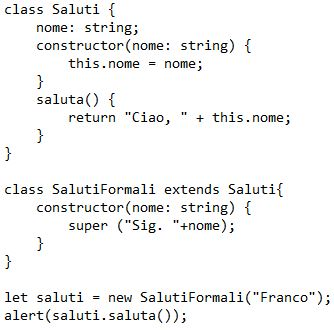
\includegraphics[width=8cm]{figure/Typescript_classi.jpg}\end{center}}
\caption{Esempio di utilizzo di classi e ereditariet\'a in TypeScript.\label{Typescript_classi}}
\end{figure}
Ammettendo le classi, TypeScript supporta di conseguenza anche il concetto di eredit\'a; nella figura ~\ref{Typescript_classi} si pu\'o vedere come la classe SalutiFormali estenda Saluti, di conseguenza ne eredita il metodo saluta().
Dal codice riportato nell'esempio si pu\'o notare come TypeScript, ammettendo le classi, semplifichi notevolmente la scrittura del codice il quale, se scritto in puro JavaScript tramite i prototipi, sarebbe molto pi\'u complesso.

\subsection{Moduli}
\begin{figure}[tp]
    {\begin{center}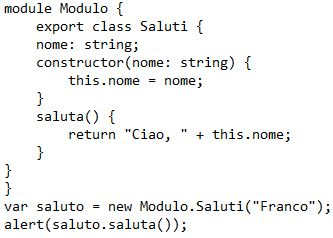
\includegraphics[width=8cm]{figure/Typescript_modulo.jpg}\end{center}}
\caption{Il codice mostra l'utilizzo dei moduli in Typescript.\label{Typescript_modulo}}
\end{figure}
Una funzionalit\'a molto apprezzata di TypeScript \'e il supporto nativo ai moduli, molto utili nella strutturazione del codice.
Nell'esempio della figura ~\ref{Typescript_modulo} si pu\'o osservare un esempio di modulo; per poter essere contenuta all'interno di esso, la classe Saluti deve essere preceduta da export, dopo di che \'e possibile accedervi dall'esterno utilizzando Modulo.Saluti.


\section{React.js}

React \'e una libreria Javascript realizzata da Facebook e Istagram con l'obbiettivo di facilitare la creazione di un'applicazione a singola pagina, fornendo una struttura che la divide in componenti dinamici e riutilizzabili.
Ogni componente React \'e una classe Javascript che estende la classe Component, la quale rappresenta un blocco atomico di codice HTML e le le sue eventuali componenti dinamiche.
I componenti sono isolato tra di loro e questo aiuta notevolmente in fase di sviluppo ad avere un codice meglio organizzato e meno caotico, in oltre facilita il riutilizzo di porzioni di codice.
Ogni componente \'e composto unicamente da metodi JavaScript tra cui il metodo render() che ritorna la parte di codice HTML da mostrare.
A differenza di molti altri linguaggi e framework, React.js non usa pattern MV* e non permette la modifica diretta del DOM; ne fornisce uno virtuale sul quale possono essere cambiati elementi dinamicamente e React provveder� a modificare quello reale in maniera efficiente e veloce.
Nonostante non si basi su pattern MV*, React \'e un linguaggio completo e performante; non implementa nativamente i router, ma sono numerose le librerie di terze parti che possono fornirli.

\subsection {Classi}

\begin{figure}[tp]
    {\begin{center}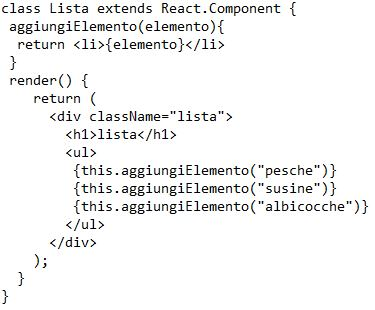
\includegraphics[width=8cm]{figure/react_componente.jpg}\end{center}}
\caption{La figura contiene una classe in React.js.\label{react_componente}}
\end{figure}

Le classi in React devono estendere React.Component e contenere il metodo render().
Come si pu\'o osservare dall'immagine ~\ref{react_component}, il metodo render ritorna le modifiche che dovranno essere effettuate nel file html; nell'esempio verr\'a creata una lista contenente tre elementi.
La loro creazione viene effettuata chiamando il metodo aggiungiElemento(), il quale restituisce il codice html corrispondente all'elemento da aggiungere nella lista.
 
\section {Angular}

Angular, comunemente chiamato Angular2+ per non confonderlo con AngularJS \'e un framework basato su TypeScript per lo sviluppo di applicazioni basate sul web.
La prima versione stabile fu rilasciata nel 2016 dal team che svilupp\'o AngularJS.
La sintassi del nuovo framework \'e completamente diversa dal suo predecessore e molti concetti chiave in AngularJS non sono pi\'u supportati.
Nel marzo 2017 Angular \'e stato aggiornato alla versione 4, per supportare le ultime versioni di TypeScript e per incrementare sensibilmente le prestazioni dell'applicazione.

\subsection {Differenze tra AngularJS e Angular}

Angular2+ adotta un approccio di User Interface di tipo component-based, perci\'o il concetto di direttive di AngularJS \'e stato sostituito dai Component.
Adottando TypeScript, questa nuova versione inserisce il concetto di classi e di conseguenza di ereditariet\'a, permette inoltre di includere nel progetto tutte le librerie di TypeScript.
\begin{figure}[tp]
    {\begin{center}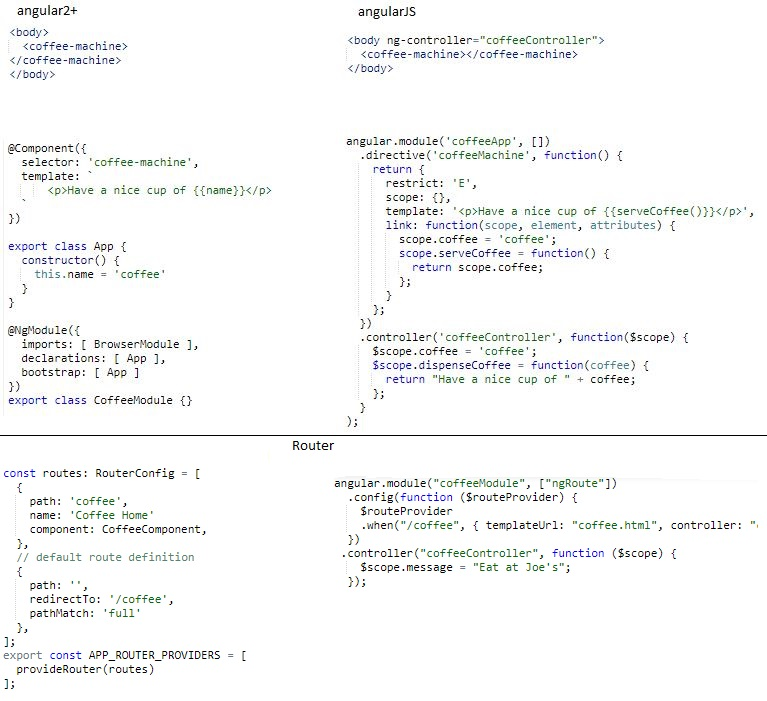
\includegraphics[width=15cm]{figure/Angular2+vsAngularJS.jpg}\end{center}}
\caption{La figura contiene porzioni di codice in AngularJS e Angular2+.\label{Angular2+vsAngularJS}}
\end{figure}

Nella figura ~\ref{Angular2+vsAngularJS} sono presenti alcune parti di codice di due semplici applicazioni identiche scritte in Angular2+ e AngularJS; si pu\'o notare come a sinistra non siano pi\'u presenti il tag ng-controller, il controller e la variabile \$scope, che vengono incapsulati nei componenti, definiti come una classe con il decoratore @Component.
Un'altra differenza sono i router; nella prima versione si utilizzavano attraverso \$routeProvider, mentre in Angular2+ si definiscono in un modulo esterno definendo il nome, il path ed il componente associato al percorso.




